% ============================================================
% 第三章 · 美学与用户体验
% 对应大纲：# 三、美学与用户体验
%
% 叙述口径：写我们最终要达到的视听标准与设计理由，不写当前完成度。
%
% 术语约定：
%   游戏名 = 《借灯》（\ProjectName）；组名 = 白灯客
%   白灯 = 故事里那盏没有火焰的纸灯笼，也是全篇唯一的暖光源
%
% 界面设计一节（站点地图 / 线框图 / 设计图）留标题，由组员自行补写。
% ============================================================

\chapter{美学与用户体验}

\section{视觉设计规范}

\subsection{整体风格}

《\ProjectName》的视觉只讲一个对比：冷夜里的那盏灯，基于强烈的冷暖对比进行设计。

故事里的白灯笼没有火焰，却在雨夜里泛着白光。它代表掩饰，在画面中被做成全篇唯一的暖光源。其余元素，雨、雾、废弃的矿区、没有窗的屋子，全部压在冷调里。玩家进入任何一个场景，视线都会先落到亮的那一点上。

这个对比同时解决了一个实际问题。全篇场景出自不同批次，祠堂在室内，矿井在地下，数据机房是现代的，如果各画各的，玩家每换一个地方都要重新适应。规范因此固定四样不变的东西：色板、雨、灯、字体。场景内容可以不同，这四样必须一致，玩家切换场景时感受到的是同一个雨夜里的不同地点。

\subsection{配色}

全站颜色收拢到一个变量文件里，其余样式表只引用变量名，不单独书写色值。这样做的目的是让配色一致性自动维持：修改一处底色，所有页面同步变化，不会出现主菜单与老宅场景相差三个色阶的情况。

\begin{table}[htbp]
\centering
\caption{全站色板}
\small
% Token 名写成 -{}-bg 而不是 --bg：xeCJK 下 \ttfamily 打开了 TeX 连字，
% 裸的 -- 会被排成破折号。
\begin{tabularx}{\linewidth}{@{}l l X@{}}
\toprule
分组 & 色块与 Token & 用途 \\
\midrule
冷底   & \swatch{cBg} \texttt{-{}-bg (\#07090e)}                & 页面最深底色，场景最暗处 \\
       & \swatch{cBgElevated} \texttt{-{}-bg-elevated (\#0d1118)} & 面板与卡片底 \\
       & \swatch{cBgElevated} \texttt{-{}-panel}                & 文本框与侧栏的半透明底 \\
\addlinespace
纸与暖金 & \swatch{cLamp} \texttt{-{}-lamp (\#f5f0e3)}           & 白灯的光，热点光晕与高光 \\
       & \swatch{cPaper} \texttt{-{}-paper (\#ece7dc)}          & 正文纸白 \\
       & \swatch{cPaperDim} \texttt{-{}-paper-dim (\#cfc8b8)}   & 次级文字、旧纸 \\
       & \swatch{cAccent} \texttt{-{}-accent (\#d8c6a4)}        & 强调暖金，木纹、旧物、描边 \\
       & \swatch{cAccentDeep} \texttt{-{}-accent-deep (\#b89b6e)} & 深金，按钮悬停态 \\
\addlinespace
冷点缀 & \swatch{cMist} \texttt{-{}-mist (\#8fb8ce)}            & 雾蓝，冷光与次级点缀 \\
       & \swatch{cRain} \texttt{-{}-rain (\#5d7f9e)}            & 雨蓝，雨丝与冷调 \\
\addlinespace
警示   & \swatch{cCinnabar} \texttt{-{}-cinnabar (\#a6534a)}    & 朱砂红，关键真相与门外的声音 \\
       & \swatch{cDanger} \texttt{-{}-danger (\#c17a74)}        & 错误与警示 \\
\bottomrule
\end{tabularx}
\end{table}

用色规则可以概括成一句：底色永远冷，强调永远暖。

朱砂红是使用限制最严的颜色，只允许出现在三处：关键真相线索、错误提示、门外那个叫名字的声音。一旦大面积使用，它就不再表示紧急，玩家对它的警觉也会随之消失。

两项可读性指标定为硬性要求：正文与背景的对比度不低于 4.5:1，最小的楷体字不小于 12px。探索区叠加在场景图上的标签必须垫一层深色半透明底，不能把浅色字直接压在亮背景上。场景图中存在高亮区域，浅色标签叠加其上会失去可读性。

\subsection{字体}

\begin{table}[htbp]
\centering
\caption{字体与字号阶梯}
\small
\begin{tabularx}{\linewidth}{@{}l l l X@{}}
\toprule
层级 & 字体 & 字号 / 行高 & 用途 \\
\midrule
标题 & 宋体 & 24px / 字距 0.18em & 游戏名、章节名、场景名 \\
正文 & 宋体 & 17--21px / 1.9 & 剧情正文、人物对白 \\
旁白与小字 & 楷体 & 12--15px / 1.6--1.8 & 说明性小字、旁白细节 \\
界面标签 & 无衬线 & 14px & 按钮、顶栏、系统提示 \\
\bottomrule
\end{tabularx}
\end{table}

宋体笔画清晰，适合长段落阅读，用于剧情正文和场景名。楷体接近手写，放在说明性小字上，与正文形成区分，避免提示文字打断阅读。按钮和顶栏需要快速识别，使用无衬线字体。

封面单独使用一套毛笔手写字体，全篇只在封面出现一次，重复使用会削弱它的辨识作用。

正文的 1.9 倍行高和标题 0.18em 的字距是依据中文排版特点设定的。中文没有词间空格，字号越大、字距越密，长句越容易读串行，行高和字距是替代空格的主要分隔手段。

\subsection{人物立绘}

立绘只有两个站位，左和右，分别落在画面两侧 5\% 的位置。哪个角色站哪边写在数据里，渲染层只读站位数值，不判断来的是谁。这样加一个人物不需要改渲染代码，改一个字段就够了。

立绘的作用是表示场景中有人在场，同一时刻只出现一个，站位的变化即表示说话人更换。

苏禾全篇不出正脸立绘，只以笔迹、照片和登记记录出现。这是因为，她的死要等到第二次汇合才揭晓，任何一张正脸立绘都会让玩家在她真正出场之前就先认出她。美术不必把每个角色都画出来，隐藏不该出现的角色同样是设计的一部分。

\subsection{美术原则}

场景图同时承担背景和线索载体的功能，美术有四条硬性要求。

\begin{enumerate}
  \item \textbf{光源统一。} 每个场景只设一处主白灯光源，位置随场景走：祠堂在门和梁上，村口在电杆和屋檐，老宅在门后。光晕半径约为场景短边的一半到七成。任何情况下不得遮住发光热点、线索和对白区。
  \item \textbf{冷暖不混。} 关键对象和热点不许埋在暖光晕里。玩家点哪一处、就看哪一处
  \item \textbf{画布与安全区统一。} 场景按 1280$\times$720 绘制，16:9，满屏不裁切。底部 600 到 720 一条留给阅读框和按钮，关键信息不往里放。
  \item \textbf{背景不许剧透。} 每张图交付前要过一遍：这张图有没有提前泄露某个人的结局、某一层身份的关系。有就改。
\end{enumerate}

这四条写进了场景交付模板，每张图由美术、剧情和前端三方逐项确认之后才能合入。氛围统一因此有了可以逐条核对的验收标准。

\subsection{动效规范}

日常动效控制到几乎不可察觉，只有三类。

雨丝垂直缓慢下移，透明度很低，不干扰阅读。白灯的光晕在 0.85 到 1 之间以约 2.5 秒的周期缓慢起伏，该效果只用在灯和发光热点上。场景切换统一使用 200 到 400 毫秒的淡入淡出，全篇不做变化。

限制强度的原因是：玩家要在这个界面上读三个小时的字，任何一处抢注意力的动效都会被反复看到几百遍。动效的作用是维持画面的活性，不是吸引玩家注意动效本身。

规范中另有一条硬性要求：动效不触发眩晕，不做大面积快速位移，并且尊重系统的减少动态效果设置。高强度的动态效果全部留给关键转场，见本章第四节。

\section{文字风格}

\subsection{整体调性}

全篇有一条硬性要求：游戏里出现的所有文字都要出自故事世界内部，不出现项目组直接对玩家说话的情况。

这一条在执行时比想象中容易破。V4 定稿时删改幅度最大的一批文案，问题几乎都出在这里。原文里有一句“恭喜你，成功解锁【陈家老宅】相关剧情”，句式上是系统提示，效果上把玩家从故事里拽了出来，让他在沉浸最深的时候意识到自己在操作一款游戏。同一批改写里还有一处“归档结论”，用文件摘要的语气替玩家把结论下完了。这两处最后都换掉了：前一句整句删除，后一句改由主角的独白提出，而且停在问句上。

判断标准可以总结成一句：结论由玩家得出，文本不替玩家下结论。

\subsection{用语}

写作时要求描述现场能直接看到、听到的东西。

改稿前有一段描述证据吻合的文案，用的是重合、证明、表明这一类词。这是文件摘要的口气，读起来像在审一份报告。改写之后变成了：纸已经很旧了，可撕口还是白的，是最近才撕开的。两句话说的是同一个判断，前一种写法要玩家自己翻译一遍，后一种写法直接把画面放到他眼前。

抽象概括会让玩家觉得自己在读材料，具体的形貌、声音、温度，才会让他觉得自己站在那个地方。

角色语言的个体差异在第二章已经展开过，这里只补充它对叙述层的要求：同一件事，村民用口语，小周用短句，主角用疑问句。叙述层不跟随任何一个人的语气，它始终是全篇最冷的那一层。

\subsection{氛围营造}

氛围的营造依靠信息的分寸，不依靠形容词。

全篇没有一句直接告诉玩家这里很吓人。与其写雨夜的村子很阴森，不如写纸上那道撕口还是白的。先给出一个具体的东西，再把它留给玩家自己去理解。

名牌制度也服务于这一点。旁白不出名牌，正文自己陈述，玩家读到的是一段没有来源的叙述；独白出名牌，那句话就被标记为主角自己的声音。两者在视觉上区分得很清楚，玩家始终知道一句话是谁说的，或者知道它没有来源。

情节里最沉重的细节，我们选择不做解释。父亲签下停止搜救那一段，处理方式是让玩家自己停下来，文本不跟任何评价。这种留白是刻意的，目的是把最后一步留给玩家自己完成。

\section{界面设计}

% 本节由组员补写，分三块：站点地图 / 线框图 / 设计图。
% 图片就位后用 \fig 插入，例如：
%   \fig[0.9]{figures/03-ux/sitemap.png}{站点地图}{sitemap}
% 站内页面清单（pages/ 目录，12 个）：
%   游戏主流程  pages/game.html
%   主菜单      pages/menu.html
%   登录 / 注册 pages/authorize/login.html、register.html
%   成就        pages/achievements/achievements.html
%   项目介绍    pages/about/project.html
%   制作组      pages/about/team.html
%   成员页 ×5   pages/about/members/{yu-zhirang,luo-chenfei,gao-bingxuan,
%               lu-zhengsong,yang-meng}.html

\subsection{站点地图}

\begin{figure}[htbp]
\centering
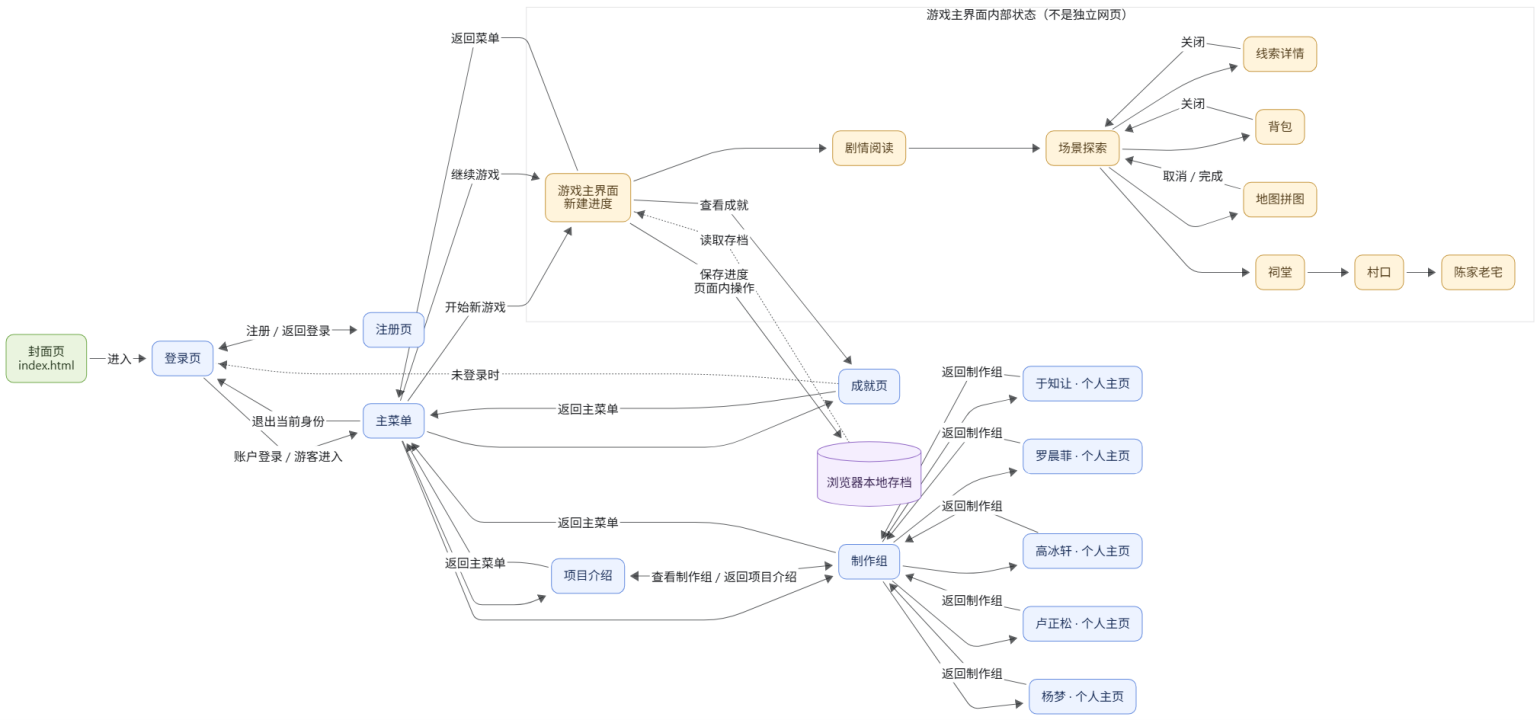
\includegraphics[width=0.9\textwidth]{figures/03-art-and-experience/locate.png}
\caption{站点地图结构}
\label{fig:locate}
\end{figure}

\subsection{线框图}

\pending

\subsection{设计图}

\begin{figure}[htbp]
\centering
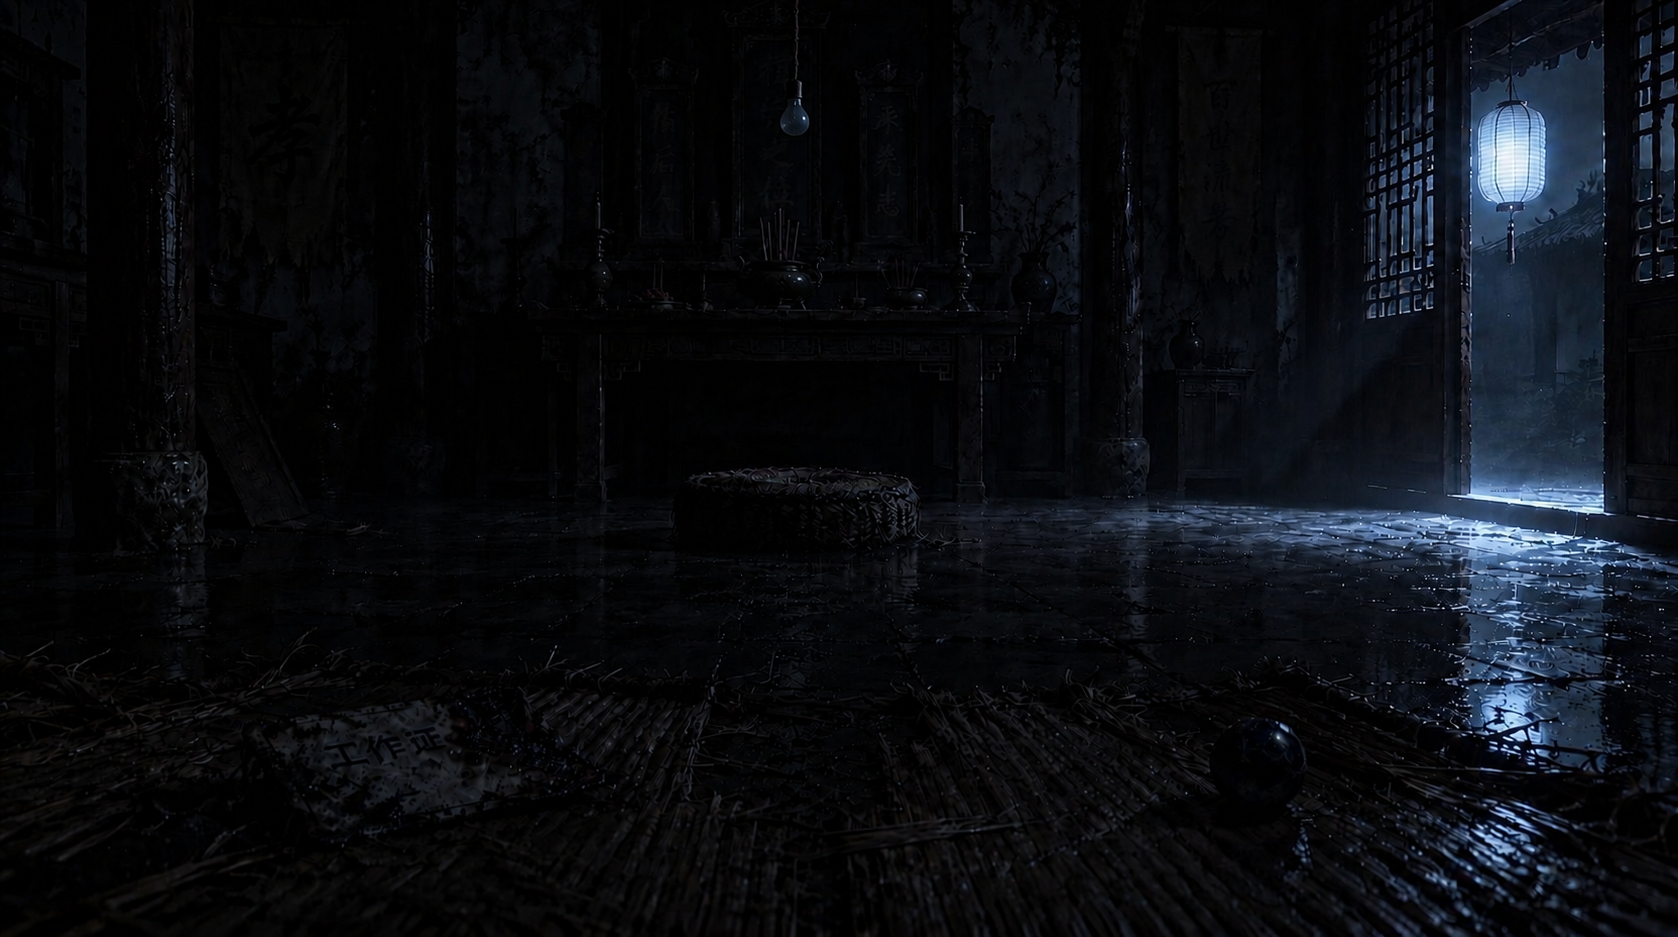
\includegraphics[width=0.9\textwidth]{figures/03-art-and-experience/lampUp.png}
\caption{祠堂灯亮设计}
\label{fig:lampUp}
\end{figure}

\begin{figure}[htbp]
\centering
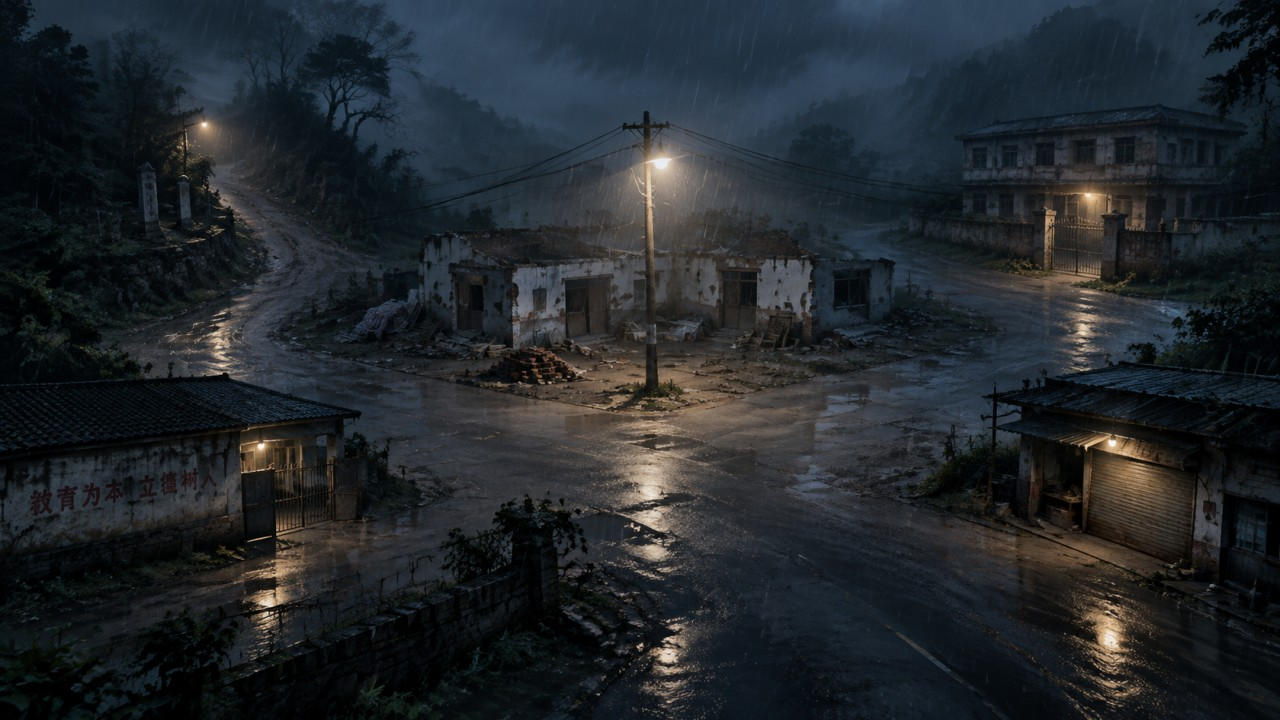
\includegraphics[width=0.9\textwidth]{figures/03-art-and-experience/outer-investigation-hub.jpg}
\caption{四条探索分支背景设计}
\label{fig:outer-investigation-hub}
\end{figure}



\section{恐怖美学设计}

\subsection{整体特点}

全篇的恐怖不使用惊吓手法。

惊吓的效果只持续几秒。我们采用的方式是持续的心理压抑：玩家玩到中段时意识到，自己刚才拆开的每一个装置，材质、颜色、声音，都来自主角小时候见过的东西。那一刻不产生惊吓反应，产生的是心理上的沉重感。

因此全篇没有突然出现的巨响，主要手法都带有一层铺垫：灯先闪两下才暗下去，声音先响画面再跟上，门外先叫一声名字，隔一拍玩家才听清那是谁。恐惧感来自预期落空的那半秒，与音量无关。

这套做法的核心是反差。玩家在前半段接受的是一套民俗禁忌的解释，中段被告知所有异象都是人为布置，此时本该放松。紧接着他会认出，布置所用的元素全部取材于主角的童年创伤，他把自己最怕的东西做成了恐吓他人的工具。恐惧的来源由外部转向人本身，并且落在玩家自己操控的这双手上。

\subsection{音效}

音效承担环境层，同时负责制造真假难辨的效果。

檐下的雨、排水渠里的水、广播里带电流杂音的童谣、远处传来的爆破回声，这几层声音持续存在。它们同时属于村庄的日常环境与恐吓装置的一部分。玩家在中段之前分不出哪一层是人为布置的，中段之后回头看，每一声都解释得通。让人不安的是玩家发现自己听了两个小时，却始终没有听出其中的区别。

背景音乐只有一条循环轨，音量控制在四成左右，切换页面时不重新起播。玩家在菜单、成就页和游戏之间来回切换，音乐不应中断。

浏览器的自动播放限制决定了第一次出声必须等待玩家的第一个操作。音频在玩家第一次点击或按键之后起播，在此之前保持静音，界面上另有一个常驻的静音开关。这项限制无法绕过，可以做的是不让它成为意外：玩家按下第一次鼠标时音乐正好响起，让它看起来是设计好的。

音频加载失败不能连带停止游戏。播放器返回失败码后，游戏降级为无声继续，控制台保留一条记录。玩家可以听不到背景音，但不能卡在黑屏前。

\subsection{视频}

过场视频用于静态画面无法交代的位置：人物的情绪转折、时间的跳跃、以及回忆片段的插入。这些位置用旁白叙述会拖慢节奏，因此交由视频承担。

全篇七段，序幕两段，五个结局各一段。

\begin{table}[htbp]
\centering
\caption{过场视频清单}
\small
\begin{tabularx}{\linewidth}{@{}l l X@{}}
\toprule
触发位置 & 素材 & 内容 \\
\midrule
序幕 · 白灯初现 & \texttt{light\_up} & 门外忽然亮起一盏灯 \\
序幕 · 祠堂断电 & \texttt{cut-off} & 祠堂内忽然断电 \\
结局一 · 交出证据 & \texttt{the\_ending} & 灯火照旧 \\
结局二 · 追逐失败 & \texttt{close\_well} & 井口又高一寸 \\
结局三 · 销毁全部 & \texttt{unnamed} & 姓名落尽 \\
结局四 · 选择性公开 & \texttt{after\_whitelamp} & 借来的黎明 \\
结局五 · 完整公开 & \texttt{no\_more\_lamp} & 此后无须借灯 \\
\bottomrule
\end{tabularx}
\end{table}

触发条件绑定在台词内容上，不绑定在剧情节点的编号上，读到对应句子才播放。这样处理在协作阶段省去很多返工：节点编号会随剧情改写而变动，如果视频绑定编号，每改一次文案就要重新核对七个编号，漏掉一个就会导致一段视频永远不播放。绑定文本之后，修改剧情不会漏掉视频，增加视频也不用改动剧情数据。每条视频只播一次。

\subsection{转场}

转场是全篇唯一使用高强度效果的位置。日常动效控制到几乎不可察觉，效果强度集中在下面这十一处。

三类基本手法，加一种抖动接闪黑的组合手法，共同点是都带有铺垫，没有一处是突然出现的。

\begin{table}[htbp]
\centering
\caption{转场手法}
\small
\begin{tabularx}{\linewidth}{@{}l l X@{}}
\toprule
手法 & 时长 & 过程 \\
\midrule
轻闪黑 & 0.9\,s & 快速压黑，短暂停顿后淡出 \\
窒息式闪黑 & 3.3\,s & 灯闪两下 $\rightarrow$ 黑幕以 550\,ms 漫上 $\rightarrow$ 黑暗中边缘红晕呼吸 1\,s $\rightarrow$ 以 1.5\,s 缓慢退出 \\
暴力抖动 & 0.65\,s & 位移从 18\,px 逐级递减到 0，叠加旋转与轻微模糊 \\
无信号花屏 & 2.1\,s & 随机噪点从画面某一点扩散到全屏，短暂停顿后收回到同一点并淡出 \\
抖动接黑 & 3.1\,s & 先抖动，120\,ms 后黑幕漫上，其余同窒息式 \\
\bottomrule
\end{tabularx}
\end{table}

窒息式闪黑中的两次灯光闪烁有明确作用。先铺垫再压黑，玩家在黑暗真正到来之前已有半秒的预感，恐惧感来自这半秒的预期落空，与黑暗本身无关。恢复阶段用 1.5 秒，比压黑慢了三倍，目的是让玩家在离开黑暗时多停留一会儿。

花屏的扩散和收束都从一个随机点开始，两次使用同一个点。收束速度慢于扩散，形成缩回原处的效果。

十一处触发同样全部绑定在台词上。一个监听器观察剧情文本的渲染结果，读到约定的句子就播放对应效果，剧情数据里不埋任何标记。这样处理的好处与视频一致：修改剧情不会漏掉转场，增加转场不需要改动剧情。

所有手法都绘制在场景层内部，与阅读区是两个独立的层。黑屏期间文本仍然存在，只是被遮住，恢复之后玩家可以接着读。全篇没有一处转场会顶掉正在显示的文字，也没有一处会接管鼠标。恐怖效果可以打断节奏，不打断操作。
